\documentclass{article} % For LaTeX2e
\usepackage{nips15submit_e,times}
\usepackage{hyperref}
\usepackage{url}
\usepackage{graphicx,float,wrapfig}
%\documentstyle[nips14submit_09,times,art10]{article} % For LaTeX 2.09


\title{Applying Convolutional Neural Networks (CNNs) for Decoding fMRI Images}


\author{
Dong Hyun Choi \\
Department of Electrical and Computer Engineering\\
Carnegie Mellon University\\
Pittsburgh, PA 15213 \\
\texttt{donghyuc@andrew.cmu.edu} \\
\And
Yongjin Cho \\
School of Computer Science \\
Carnegie Mellon University \\
Pittsbrugh, PA 15213\\
\texttt{ycho1@andrew.cmu.edu} \\
}

\newcommand{\fix}{\marginpar{FIX}}
\newcommand{\new}{\marginpar{NEW}}
\def\code#1{\texttt{#1}}

\nipsfinalcopy % Uncomment for camera-ready version

\begin{document}


\maketitle

\begin{abstract}
We attempt to create a machine learning model using fMRI images that can predict which word the brain state is representing across all human subjects. Our baseline logistic regression model and neural network model achieves high mean accuracy when preprocessing the base images with linear discriminant analysis (LDA). The initial prototype of our target CNN model yields a prediction rate no better than chance, though future CNN models proposed in this paper is believed to perform better based on what we learned through the series of experiments.
\end{abstract}

\section{Introduction}

Functional magnetic resonance imaging (fMRI) is a brain imaging technology that enables us to know which part of the brain is active at any moment of a given task. Beyond trying to identify which brain region relates to certain tasks, there have been numerous attempts at trying to interpret the brain's activation state given the fMRI of itself. Specifically, Mitchell et al [1] has showed that machine learning algorithms could be used to predict what object the brain was thinking of based on fMRI images depicting voxel activations at a given time. Further researchers, such as Ramish [2], have also tried at developing cross-subject interpretation of fMRI images by using cross-subject clustering to improve the accuracy.

Convolutional neural network (CNN) is a recent technology that has shown good performance in various image analysis tasks such as image recognition and video recognition. Therefore, we attempt to use CNN as our main model in this paper to infer the state of the brain from a set of fMRI images. Though the task of inferring the brain's state from these images could be regarded as a simple extension of previous image classification examples, the fact that fMRI images are 3-dimensional and that fMRI images across people can be different for the same task provides various challenges. For example, voxel activations while thinking of a certain object will differ depending on the person being inspected. We have chosen CNN as our main model because we believe that CNNs will be able to extract general features from brain images that will help at providing better interpretation across all human subjects.

Our main goal through the various experiments is to find the best model that can provide the highest accuracy for predictions across subjects. In order to see the relative performance of our CNN model, we first implement two baseline approaches: a logistic regression model and an artificial neural network model. We then compare the results of the baseline approaches to those of the CNN based approach and explain what could be the cause of the difference in those performances.

For this midterm report, we include the details of our completed baseline approaches and the prototype of our CNN model. We also explain the base dataset, how feature extraction was done from the dataset, the structures of our models, and the various problems that we've approached. We finish the paper by showing the performances of the different approaches and the project direction for the rest of the semester.  

\section{Dataset}

\subsection{Base Dataset}

The base dataset includes nine sets of fMRI images, where each set corresponds to each unique human subject. Each image was taken while showing the subject a line drawing of one of the 60 concrete objects across 12 semantic categories. The set of objects were shown six times in random order, creating a total of 360 trials per subject. All fMRI images were normalized into MNI space and then resampled to units of 3-by-3-by-6 $mm^3$ voxels.

This dataset is organized into nine separate files, where each file contains data for a single subject. Each file has fields that include the following info:
\begin{itemize}
	\item \textbf{META}: identifier of subject, number of trials, number of voxels activated during entire trial, range of each dimension, mapping info from voxel coordinate to voxel column in \textbf{DATA}, inverse mapping info
	\item \textbf{INFO}: word (stimulus), semantic category of stimulus, number of times the stimulus was presented
	\item \textbf{DATA}: actual voxel data for all 360 trials (data dimension stated in \textbf{META})
\end{itemize}

\subsection{Preprocessed Dataset}

For our purpose of training the baseline models, the base dataset had to be preprocessed due to the irregularity of the number of voxels across all subjects. As the number of activated voxels for each subject were independent from one another, each image was first flattened into a 1-by-$n$ feature vector, where $n$ is the number of activated voxels each person has. This was then normalized so that all vectors could have the same dimension $n'$. The value of $n'$ was chosen by the maximum number of voxels there could be inside one fMRI image. This could be determined from the meta info \code{dimx}, \code{dimy}, and \code{dimz} that states the range of each dimension. When normalizing each vector, the \code{colToCoord} meta info was used to map each value in the 1-by-$n$ vector to the new normalized 1-by-$n'$ vector. Since $n' > n$, all points where no \code{colToCoord} was given were initialized to zero. This eventually created a default set of feature vectors with a dimension of $51 \cdot 61 \cdot 23 = 71553$.

The second set of feature vectors was extracted by applying principal component analysis (PCA) to the data matrix $X$, where $X$ was created by stacking the feature vectors vertically as column rows. Thus, the $i_{th}$ row in $X$ would be a 1-by-71553 vector depicting the $i_{th}$ fMRI image from the original dataset. We used only the first 200 principal components and projected all data onto these. This yielded each data instance's feature to be a 1-by-200 vector.

The last set of feature vectors was extracted by applying linear discriminant analysis (LDA) to the same data matrix $X$ that was used for applying PCA. Class labels were also provided along with the data when applying LDA, where each class label was a mapping from the 60 words that subject was tested on to a number within the range of 0 to 59. This eventually reduced the dimension of each feature vector from the original 71553 to 59.

\section{Baseline Approaches}

The task for each baseline model is to predict the word of the object that the subject was shown when the fMRI image was taken. A random choice would provide an accuracy of $1.67\%$, which is the probability of choosing one out of 60 possible candidates. All three types of feature vectors were tested to see which set of feature vectors would give the best accuracy and performance.

\subsection{Logistic Regression}

We implemented a multinomial logistic regression with L2 regularization and used gradient descent for optimizing the parameters. 

For evaluation of the classifier's performance, nine evaluations were performed such that for every $i_{th}$ evaluation, all  data except for the $i_{th}$ subject's data would be used as the training set. The accuracy of the classifier was evaluated on the unused $i_{th}$ subject's data. The average of all nine evaluations was used as the final reported accuracy.

For the classifier, we used all three types of features described in Section 2.2. The results are provided in Section 5 along with the performances from other approaches.

\subsection{Artificial Neural Network}

An artificial neural network (ANN) was created by using two hidden layers, where each layer has 1024 hidden ReLUs. A dropout rate of 50\% was used on the last hidden layer, and the total loss was additionally penalized by the sum of all losses from the weights and biases.

When evaluating the classifier's performance, the identical process from the logistic regression experiment was followed, resulting in a total of nine evaluation rounds. The details of these results can also be found in Section 5. 

For the ANN classifier, only the LDA and PCA feature sets described in Section 2.2 were used. When using the base 1-by-71553 feature set as input, the loss quickly aggregated to a large number after each gradient descent iteration, and this led to a NaN value as the total loss. As each 1-by-71553 feature vector was a sparse vector with an average of two-thirds of the elements being zero, we concluded that the results from using PCA and LDA was sufficiently enough to be used as a baseline.

\section{CNN Approaches}

We apply the same task that was used for the baseline models to the CNN model, which was to predict the word from the fMRI image. Three different experiments are proposed in order of expected performance improvements. For the first two experiments, we use the same CNN structure which consists of two convolutional layers, two pooling layers, and a fully connected layer at the end. ReLUs were used to represent each hidden layer, as ReLUs have the nice property of not requiring the input to be normalized in order to prevent them from saturating [3]. Hyperparameters were set to start with a stride of two $(S=2)$, a receptive field size of 5 x 5 $(F=5)$, a slice depth size of 16 $(K=16)$, and a padding size of zero $(P=0)$. These initial hyperparameters are based on the CNN structure that is most popularly used for MNIST demos [4], as the image dimensions of our brain images (23-by-61, 23-by-51, or 61-by-51) were not significantly different from that of the MNIST images (28-by-28). Only the first proposed experiment has been fully tested at the time of this report.

\subsection{Ensemble of CNNs With Voting}

As our CNN structure was created to mainly deal with 2-dimensional images, the original 3-dimensional data was split into sets of 2-dimensional images along each $x$, $y$, and $z$ axis to match the input format that the model requires. Three separate CNN models were created to process data from each axis, and the final prediction was determined by the vote from all three. Figure 1 shows the ensemble of the three CNN models. When all three models predicted different labels, the prediction with the strongest confidence rate was chosen as the tie breaker.

\begin{figure}[h]
	\centering
	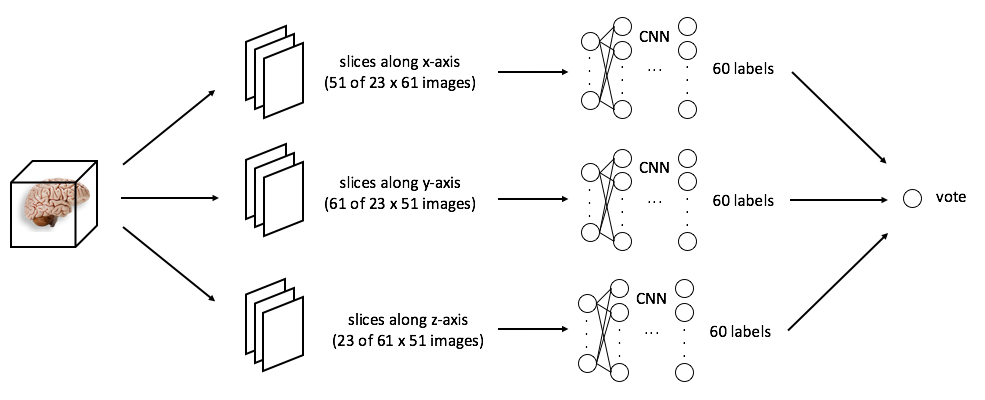
\includegraphics[height=0.26\textheight]{./img/cnn_proto_a.png}
	\caption{Structure of an ensemble of CNNs by predicting the final label through voting.}
\end{figure}

However, each CNN model reported very low accuracy for their label prediction, where the accuracy was no different from choosing the label at random. As each CNN model was not performing reasonably, the end vote consequently could not yield any useful meaning. One possible reason for the low accuracy is that we did not use the info of where each slice is physically located. Even though the slice images from a certain axis will all look radically different from one another within a single trial, the model would try to force the prediction of all of these to be one label. We provide additional analysis of the possible causes of this performance in Section 5.

\subsection{Ensemble of CNNs With Connected End Layers}

Since the three separate CNN models from the former experiment cannot learn from an error made after the voting occurs, we plan to adjust the structure so that all models are connected through one end layer. Figure 2 shows the enhanced ensemble of CNNs that are connected to one layer at the end. We believe that this will propagate errors properly when one model predicts a label that is far from what the others predict. Also, in order to accommodate the info of the physical location of each slice, we plan to add additional nodes that will propagate this information.

\begin{figure}[h]
	\centering
	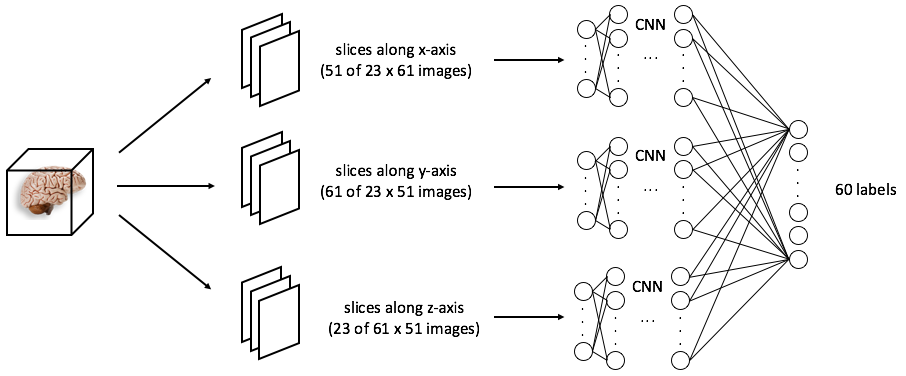
\includegraphics[height=0.26\textheight]{./img/cnn_proto_b.png}
	\caption{Structure of an ensemble of CNNs by connecting all end layers.}
\end{figure}

\subsection{3-dimensional Convolutional Layers}

We believe that a single CNN model that can stride along all three axis will perform the best, as all adjacent values in the 3-dimensional space will be used when extracting features for each receptive field. Figure 3 shows a rough structure of how this experiment will be carried out. The method for dealing with 3-dimensional images is currently being researched at the point of this report, though we think some plausible methods may be to treat underlying layers as channels or modify the pooling process by using 3-dimensional windows.

\begin{figure}[h]
	\centering
	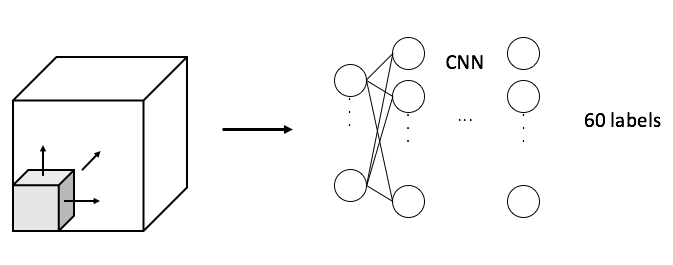
\includegraphics[height=0.2\textheight]{./img/cnn_proto_c.png}
	\caption{Structure of a CNN with 3-dimensional convolutional layers.}
\end{figure}

\section{Results}

The final results in this section are evaluated by taking the mean of nine evaluation rounds as mentioned in Sections 3.1 and 3.2. Each evaluation round rotates the subject to be used as the test set and sets all other subject's data as the training set.

\begin{table}[H]
\centering
\caption{Logistic Regression}

\begin{tabular}{|c|c|}
\hline
\textbf{Feature Type} & \textbf{Accuracy} \\ \hline
Basic                 &          1.6\%         \\ \hline
PCA                   &           6.2\%        \\ \hline
LDA                   &            90.7\%       \\ \hline
\end{tabular}
\end{table}

Table 1 shows the different performances of the logistic regression model based on what type of feature vector set is used. Using the base feature set resulted in a mean accuracy of $1.6\%$. The mean accuracy achieved by using the PCA feature set was $6.2\%$, and the mean accuracy achieved by using the LDA feature set was $90.7\%$.

\begin{table}[H]
\centering
\caption{Artificial Neural Network}
\label{my-label}
\begin{tabular}{|c|c|}
\hline
\textbf{Feature Type} & \textbf{Accuracy} \\ \hline
PCA                   &          1.7\%         \\ \hline
LDA                   &         89.0\%          \\ \hline
\end{tabular}
\end{table}

Table 2 shows the performance of the artificial neural network model when tested on only the PCA and LDA feature sets. The ANN trained with the PCA set gave a $1.7\%$ mean accuracy, while the ANN trained with LDA set gave a $89.0\%$ mean accuracy. Running the model with the basic set of $n$-by-71553 feature matrix created an overflow in the loss value, and thus could not be trained properly. We suspect the cause of the overflow to be the high dimension of the 1-by-71553 feature vector multiplied by the high number of ReLUs in our hidden layer leading to a big loss calculation.

\begin{table}[H]
\centering
\caption{Convolutional Neural Network}
\label{my-label}
\begin{tabular}{|c|c|}
\hline
\textbf{Feature Type} & \textbf{Accuracy} \\ \hline
2-d Slice                 &      1.7\%             \\ \hline
\end{tabular}
\end{table}

In Table 3, we show the performance of the first CNN experiment using 2-dimensional image slices from each trial as the input. The reason for the bad performance may be that each image slice along one axis could show many or small number of voxels based on where that slice is physically located. A slice towards the end of the brain would not contain many voxels in the first place, while the slice at the middle of the brain would contain the maximum number of voxels possible. However, the model from the first experiment treats all of these as equal data instances from a particular label. As the training data in this case is essentially saying that any voxel activation combination can be treated as one label, the amount of variance would be too high for the model to learn a proper classification. We plan to overcome this hindsight through future experiments suggested in Section 4.2 and 4.3.

\subsection{Qualitative Evaluation}

Our baseline approaches from the logistic regression model and artificial neural network model show that the basic sparse feature vector representation gives very small benefit to be used as a feature set. In contrast, when we projected the basic feature vectors onto principal components to retrieve the PCA feature sets, the performance for both baseline models improved. Still, the accuracies based on the PCA feature sets were not significantly better than those based on the basic feature sets since it remained to be lower than $10\%$.

On the other hand, both baseline models showed significantly improved accuracies when using the LDA feature sets. The reason for this could be that LDA tries to extract features that best separates the data based on the given class labels, whereas PCA doesn't consider anything about which label the data belongs to [5, 6]. Also, although the mean accuracies for both baseline models were relatively high at $90\%$, we observed that the accuracy across the evaluation rounds fluctuated between a high value of $100\%$ to a low value of $70\%$. Therefore, we think that there is no strong evidence to believe that the baseline models using LDA features are yet generalizable and applicable for cross-subject predictions.

Regarding the performance of the first CNN experiment, we suspect another reason for such low accuracy to be the way of how we defined our input features. By taking a 2-dimensional slice from a 3-dimensional voxel and treating each 2-dimensional slice to be independent from the other slices, we didn't utilize the fact that a certain slice from one axis could be strongly correlated to a different slice from another axis within the same trial.

\section{Directions for the Rest of Semester}

Based on our first CNN experiment, we plan to carry out the the latter two experiments by applying what we have learned. The proposed CNN models for future experiments will be tested to see whether they can accommodate any correlational information or physical locality. Additional enhancements being considered is to preprocess the image as how we've done so from the PCA or LDA methods, which could help normalize each image while saving all relevant details.

\section*{References}

\small{
[1] T. Mitchell \& S. Shinkareva \& A. Carlson \& K. Chang \& V. Malave \& R. Mason \& M. Just. (2008) Predicting Human Brain Activity Associated with the Meanings of Nouns. {\it Science Vol. 320, Issue 5880, pp. 1191-1195}

[2] J. Ramish. (2004) {\it CMU Summer Undergraduate Project Report}

[3] Alex Krizhevsky \& Sutskever, Ilya \& Geoffrey E. Hinton. (2012) ImageNet Classification with Deep Convolutional Neural Networks. {\it Advances in Neural Information Processing Systems 25}

[4] Y. LeCun \& L. Bottou \& Y. Bengio \& P. Haffner. (1998) Gradient-Based Learning Applied to Document Recognition. {\it Proceedings of the IEEE, 86(11):2278-2324}

[5] R.O. Duda \& P.E. Hart \& D. Stork. (2000) Pattern Classification. {\it Wiley}

[6] K. Fukunaga. (1990) Introduction to Statistical Pattern Classification. {\it Academic Press, San Diego, California, USA}
}

\end{document}